\part{Recherche préliminaires}

\chapter{Une approche méthodologique sur l'histoire des sciences}
%wrong title 
 L'histoire des sciences sociales commence par des questions existentielles sur la nature humaine et la société humaine, et les premiers chercheurs à poser les bases de ces questions furent Platon et Aristote. « L'histoire des sciences est une discipline ancienne, mais relativement récente. »\footnote{\cites{daston}} Cependant, ce n'est qu'au XVIIIe siècle, avec l'émergence de la période des Lumières\footnote{\cites{canada}}, avec de grands penseurs tels que Montesquieu, Rousseau, Voltaire, et leurs idéologies innovantes sur les sciences politiques et sociales, que les frontières entre les sciences ont commencé à devenir distinctes, et que les sciences ont été étudiées de manière différenciée.

Le XXe siècle, marqué par l'essor des méthodes de recherche quantitatives et des approches de recherche multidisciplinaires, a ouvert de nombreuses nouvelles voies dans le domaine des sciences sociales, notamment en sociologie et en anthropologie. Parallèlement, les méthodes statistiques ont permis une analyse rigoureuse des phénomènes sociaux, et ces outils ont également été utilisés pour comprendre la nature de la science et de ses organisations.

L'étude de l'histoire des sciences en elle-même, "Depuis Auguste Comte qui est considéré comme le fondateur de l’histoire de la science au début de 17e siècle", Selon George Sarton (1884-1956), le chercheur suivant est honoré comme l'un des plus grands historiens des sciences et a hérité des idéologies de Comte, telles que "qu’il est indispensable d’étudier l’évolution des sciences pour comprendre le développement de la pensée humaine, et l’histoire même de l'humanité; que c’est l’histoire de la science tout entière qu’il importe de connaître, et non l’histoire d’une ou de plusieurs sciences déterminées".\footnote{\cites{911}}. 

D'après diverses lectures sur les méthodes théoriques pour une recherche sur l'histoire des sciences, nous avons décidé d'adopter les notions fondamentales de George Sarton afin de poursuivre une étude structurée. Ses opinions et ses poursuites soulignent son engagement à documenter objectivement le développement de la pensée et de la pratique scientifiques, ainsi que les liens entre les connaissances humaines à travers les cultures et les époques.

« L’historien de la science ne doit pas se contenter d’étudier de quelles manières les sciences n’ont cessé de réagir les unes sur les autres, il doit aussi analyser les interactions qui se sont constamment produites entre les idées scientifiques et les autres phénomènes intellectuels ou économiques. »\footnote{\cite{sarton}} 

Dans le cas du Bulletin de la Société des Études Indochinoises, cette revue scientifique s'inscrit au cœur du contexte colonial, au centre des influences politiques, économiques et sociales entre les trois pays d'Indochine et l'empire français. Par conséquent, les facteurs environnementaux qui entourent cette société savante et sa revue sont essentiels pour une meilleure compréhension de celle-ci.

Ses axes de recherche tournent autour de l'analyse chronologique, de la perspective interculturelle, des études biographiques, de l'évolution des institutions scientifiques, de l'analyse des sources primaires, de l'historiographie des sciences, et toutes ces orientations sont héritées et développées dans les études des sciences modernes.

Sarton constate que « l’histoire de la science a pour but d’établir la genèse et l'enchaînement des faits et des idées scientifiques, en tenant compte de tous les échanges intellectuels et de tous les influences que le progrès même de la civilisation met constamment en jeu. »\footnote{\cite{sarton}}

La science repose sur les flux de partage, les échanges intellectuels, et les archives scientifiques coloniales constituent un exemple de ce que l'on pourrait appeler une « migration scientifique » d'un continent à l'autre (de l'Europe vers l'Asie) et de la France vers l'Indochine. Grâce aux recherches menées à partir des données de la revue, le B.S.E.I. promet d'ouvrir des perspectives plus précises sur cette circulation intellectuelle.

« Enfin, l’historien de la science entière nous permet seul, d’apprécier justement l’évolution scientifique à une époque ou un milieu déterminé. Il est arrivé souvent, en effet, qu’une science a cessé d’être cultivée, tandis qu’une autre progressait, ou bien que la culture scientifique se déplaçait dans l’espace, émigrant d’un peuple à l’autre .»\footnote{\cite{sarton}}

Le B.S.E.I. est une revue scientifique interdisciplinaire couvrant les sciences fondamentales, et elle est contemporaine de la création des fondations de recherche de Sarton au début du XXe siècle. Ainsi, les domaines d'intérêt de la revue ont également des points communs similaires avec ses orientations de recherche.

De plus, alors que l'historien s'intéresse à l'étude de chaque discipline scientifique distincte, les chercheurs des sciences se sont de plus en plus concentrés sur \textit{les approches interdisciplinaires}. Ce sont des « aspects de l’interdisciplinarité considérée comme un processus d’intégration des disciplines en même temps que d’évolution paradigmatique »\footnote{\cite{appro}}.

Nous pensons également que les approches multidisciplinaires sont particulièrement utiles. Avec une source de données telle que le B.S.E.I., il est nécessaire d'adopter une perspective pluridimensionnelle. Cela signifie considérer à la fois la revue et la société savante comme des institutions scientifiques avec des éléments de leur mécanique administrative, ce qui concerne l'histoire des sciences. En même temps, il est important de les situer dans un contexte colonial et multiculturel lié à l'histoire coloniale. Enfin, l'utilisation d'outils numériques quantitatifs permet d'aborder les aspects possibles de manière plus approfondie.

L’intersection de la science avec des connaissances issues d'autres domaines tels que la philosophie, la sociologie, l’anthropologie et l’histoire de la technologie permet de mieux contextualiser le développement scientifique. Un autre axe de recherche est l'histoire culturelle et sociale des sciences, qui prend en compte le contexte social et culturel dans lequel la science émerge et se développe, approfondissant ainsi l'étude. Ces facteurs sociaux, notamment politiques, économiques, religieux et de genre, influencent la production et la réception des connaissances scientifiques. En particulier, notre recherche se concentre sur l'utilisation des humanités numériques et des nouveaux outils de recherche pour réinventer la science elle-même. Les progrès des humanités numériques, le développement continu de l'intelligence artificielle, la formation de scientifiques multidisciplinaires et l'accès aux documents historiques numérisés ont facilité l'adoption de nouvelles méthodes de recherche et d'analyse des données dans l'histoire des sciences. Les chercheurs peuvent désormais mener des études à grande échelle basées sur des données.

Au cours des dernières décennies, les avancées en analyse numérique, ainsi que l'ouverture de nombreux projets de numérisation de documents, y compris des documents coloniaux réalisés à grande échelle tels que le DARIAH (Digital Research Infrastructure for the Arts and Humanities), ont encouragé la création de sous-projets de numérisation des documents coloniaux. Par exemple, Colonial Despatches contient la correspondance officielle entre les gouverneurs des colonies de l'île de Vancouver (1849-1866) et de la Colombie-Britannique (1858-1871) avec le British Colonial Office, tandis que CAROAT (Colonial Records of East and West Africa) comprend des documents de l'époque coloniale britannique de l'Afrique de l'Est et de l'Ouest, et ainsi de suite.

Récemment, de nombreuses recherches en humanités numériques ont été appliquées aux archives coloniales pour reconstituer des événements passés à l'aide d'ordinateurs. Certains projets intéressants comprennent, par exemple :

\textbf{Voyages: The Trans-Atlantic Slave Trade Database} : une base de données hébergée à l'Université Rice qui a pour objectif de présenter l'ensemble du matériel documentaire relatif à la traite transatlantique des esclaves\footnote{\cite{slave}}

\textbf{Vistas: Visual Culture in Spanish America, 1520-1820} (La culture visuelle de l'Amérique espagnole), également connue sous le nom de culture visuelle coloniale ou culture visuelle vice-royale, cette période s'étend sur trois siècles, allant d'environ 1520 à 1820..\footnote{\cite{visual}}

\textbf{Nahuatl/Nawat in Central America} \footnote{\cite{nana}} Les archives numériques Nahuatl/Nawat en Amérique centrale : (en espagnol, El Náhuatl/Náhuat en Centro América, ou NECA) rassemblent un corpus de textes manuscrits de l'époque coloniale produits en Amérique centrale dans des variantes des langues mésoaméricaines apparentées, notamment le nahuatl et le nawat.

Cette recherche n'est pas en dehors du courant actuel de recherche sur les traces coloniales, mais s'inscrit uniquement dans le cadre des premières découvertes de sources coloniales indochinoises.

\textbf{Remarque} : La revue B.S.E.I se consacre au thème de l'Indochine dans son ensemble, mais cette étude se penchera plus spécifiquement sur le Vietnam, en particulier sur la Cochinchine, par rapport aux régions du Laos et du Cambodge. Cette focalisation découle en partie des limites de la compréhension de ce sujet par chaque chercheur, ainsi que des données indiquant que le Vietnam maintient constamment le ratio de population le plus élevé parmi les trois pays. De plus, les recherches actuelles menées par le magazine B.S.E.I. sont également davantage orientées vers le Vietnam.

Les estimations françaises, vers 1870 \footnote{\cite{paris_2016}}, donnent :

\begin{itemize}
    \item Cochinchine : deux millions d'habitants
    \item Tonkin : quatre millions d'habitants
    \item Annam : trois millions d'habitants
    \item Cambodge : un million d'habitants
    \item Laos : de 700 000 à 800 000 habitants
\end{itemize}

\section{La science traditionnelle indochinoise}

« Du latin classique, le mot scientia est passé dans le latin chrétien. S. Jérôme l’emploie en traduisant la Bible, que ce soit l’Ancien ou le Nouveau Testament, pour désigner la connaissance donnée par Dieu aux créatures : [Deus] dat sapientiam sapientibus, et scientiam intelligentibus disciplinam, « [Dieu] donne aux sages la sagesse et la science à ceux qui savent discerner »" \footnote{\cite{science}}

Cette notion occidentale est traduite en langue vietnamienne sous le terme « khoa hoc », défini dans le Dictionnaire Han Viet tu dien (1930) comme « un ensemble d'études formant un système », et il est considéré comme faisant partie du mot « khoa cu », qui désigne le système des concours royaux pour sélectionner les mandarins.\footnote{\cite{khoa}}. Ce terme est traduit une deuxième fois à partir du chinois classique, car le mot « khoa » lui-même est également un emprunt du chinois.

À ce jour, le mot « science » est également utilisé comme adjectif, indiquant l'ordre et la systématicité, impliquant la standardisation et la modération dans la vie. Par exemple, on peut dire « Anh ay song rat khoa hoc », ce qui signifie littéralement "Il vit très scientifiquement" en français.

Une définition relative de ce mot en Vietnamien « vivre scientifiquement est une méthode de vie scientifique et raisonnable, axée sur les habitudes de vie, d’alimentation et d’exercice. »\footnote{\cite{khoahoc}}
Cette analyse met en évidence comment l'introduction de concepts scientifiques, depuis la période coloniale jusqu'à nos jours, a sensiblement élargi la portée et l'intégration du terme au sein de la société vietnamienne. Ce terme est devenu un adjectif couramment utilisé, bien qu'il ne partage pas nécessairement la même acception académique que le mot « science » mentionné précédemment. Pour mieux comprendre ce phénomène, il est pertinent de revenir à l'époque précoloniale en Indochine et d'examiner la conception de la science à cette époque. Pour ce faire, nous commencerons par étudier les premiers moyens de transmission de la connaissance, notamment la tradition orale.

\begin{figure}
    \centering
    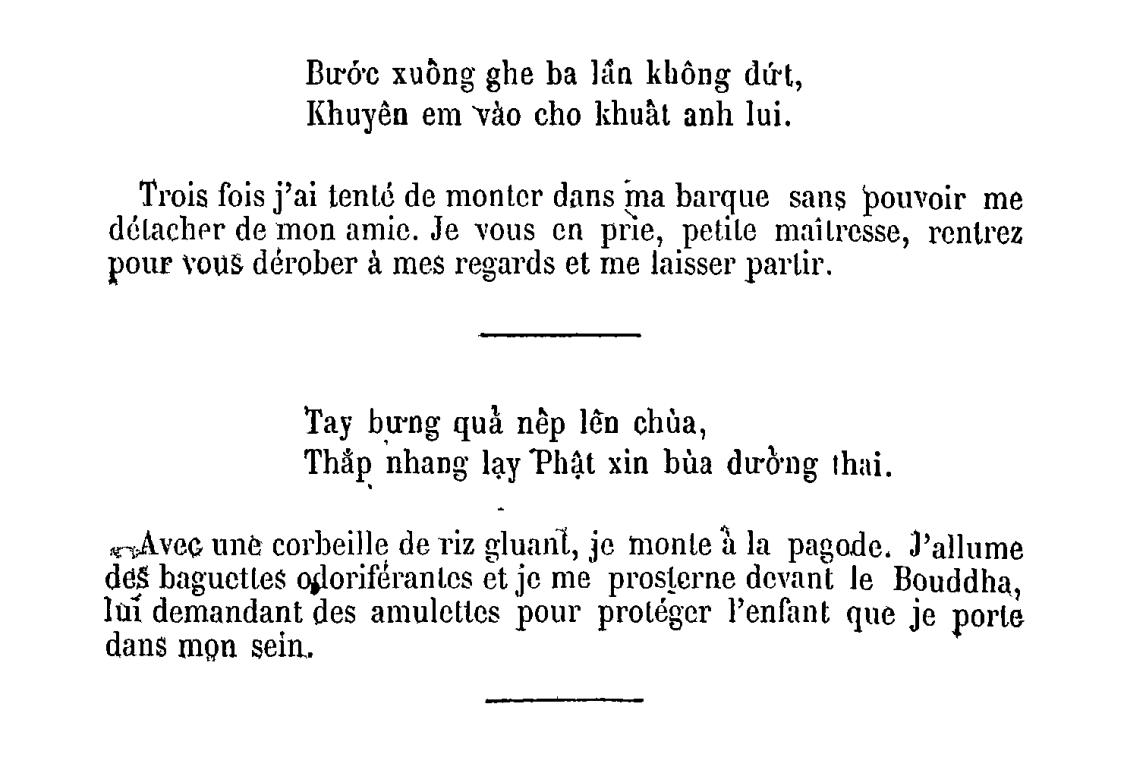
\includegraphics[width=1\linewidth]{img/1896.PNG}
    \caption{Chantes populaires et proverbes annamites} \footnote{\cite{cadao}}
    \label{fig:1896}
\end{figure}
Les chants populaires vietnamiens ont été traduits et présentés pour la première fois dans le Bulletin de la Société des Études Indochinoises en 1896 (voir figure \ref{fig:1896}). Avant l'apparition de l'écriture et encore aujourd'hui, les Vietnamiens ont une habitude culturelle de transmettre des connaissances de manière orale et de se souvenir de chants populaires (ca dao) et de tuc ngu (proverbes) pour communiquer des messages, des leçons de morale et des expériences agricoles dans la vie quotidienne. 
Comme dans de nombreux pays, la littérature orale et populaire précède souvent, voire toujours, la littérature écrite. Ces phrases, ces chansons et ces écrits sont transmis de bouche à oreille, de génération en génération, sans que l'on sache de nos jours qui en était l'auteur authentique. »\footnote{\cite{tinh}}
Dans un numéro du B.S.E.I de l'année 1963, un article décrit la science au Vietnam.

« Dans l'ancien Vietnam, la science expérimentale, telle que nous la concevons en Europe, n'a pour ainsi dire pas existé. Ce phénomène était d'ailleurs général en Asie, et la Chine, comme l'Inde, jusqu'au contact avec les Occidentaux, possédaient surtout une science empirique et des techniques traditionnelles. La culture chinoise, guère différente de la culture du Moyen-âge européen, accordait une place privilégiée et prépondérante à la littérature, à la philosophie et à la morale »\footnote{\cite{bsei}}

La transmission du savoir et de la culture dans les régions du Vietnam, du Laos et du Cambodge a une histoire profondément enracinée, débutant principalement par une tradition orale. L'éducation traditionnelle trouve son foyer dans les temples bouddhistes et confucianistes, particulièrement dans le nord du Vietnam. Les moines et les érudits de ces temples, vénérés en tant que sages respectés, se consacraient à l'étude des écrits en chinois, qui étaient la langue des textes classiques avant l'avènement du chu-nom et de la romanisation vietnamienne. Ces érudits, tout en étant des gardiens du savoir, étaient également des statues de moralité symbolique. Ils étaient étroitement liés à la communauté et à la population locale. Le tout premier établissement universitaire au Vietnam était le Temple de la Littérature, lui-même un temple confucianiste.

Au Vietnam, il existait également des enseignants privés qui dispensaient des cours particuliers, principalement destinés aux étudiants masculins, en vue de les préparer aux examens organisés par la cour royale. Ces examens visaient à conférer des titres pour occuper des postes gouvernementaux impériaux. Ces examens portaient principalement sur « Văn » (y compris la littérature, la philosophie, la morale), c'est pourquoi les intellectuels vietnamiens sont également désignés sous le terme de lettrés. Ces pratiques représentaient les manifestations majeures de la compétition intellectuelle dans la tradition confucéenne. Les influences de la culture chinoise, de l'astronomie et du calendrier lunaire étaient également omniprésentes et appliquées, en particulier dans le domaine de l'agriculture, notamment la culture du riz. 
Les régions montagneuses et les collines du Vietnam, couvrant une grande partie de son territoire, ont vu l'émergence de techniques sophistiquées de terrassement et de systèmes d'irrigation adaptés aux rizières.

La classe intellectuelle et l'élite au Vietnam étaient fortement influencées par la culture chinoise, maîtrisant les caractères chinois et adoptant les idées confucéennes. En plus de leurs rôles d'intellectuels, ils occupaient des postes de haute importance au sein du gouvernement en tant que mandarins, tout en nourrissant un fort patriotisme et un engagement envers leur patrie. Malgré près d'un millénaire de domination chinoise, le Vietnam a réussi à préserver sa culture et sa langue distinctives, même en face de nombreuses influences culturelles.

Le confucianisme, adopté en harmonie avec les croyances bouddhistes et les rituels ancestraux, a joué un rôle essentiel dans la construction de l'identité nationale et de la moralité au Vietnam. Le culte des ancêtres, le bouddhisme et le confucianisme ont renforcé les valeurs idéologiques et morales de la société vietnamienne. De plus, des croyances religieuses telles que le taoïsme et le caodaïsme, propres au peuple vietnamien, ont également émergé. La langue nationale a également joué un rôle essentiel dans la formation de l'identité nationale.

Au Laos et au Cambodge, deux pays majoritairement bouddhistes Theravāda, les moines occupent une place centrale dans l'enseignement, en particulier pour la langue principale, le khmer, et la médecine. Les monastères servent de centres éducatifs et religieux.

En ce qui concerne l'architecture et l'ingénierie, notamment les monuments d'Angkor au Cambodge, les palais et les pagodes, un niveau élevé de compréhension professionnelle et mathématique était requis. L'Indochine a connu un développement rapide de l'agriculture, en particulier de la culture du riz. Le climat tropical, caractérisé par des pluies abondantes, une chaleur constante et une humidité élevée, favorise une croissance rapide des plantes, bien que les risques climatiques soient également fréquents. Pour cette raison, les savoirs agricoles, fondés sur l'observation des étoiles et des cycles lunaires sont importants.

Les régions du Vietnam, du Laos et du Cambodge ont une histoire riche et complexe de transmission du savoir et de la culture, ancrée dans des traditions orales, des institutions religieuses, et des pratiques agricoles sophistiquées. Ces sociétés ont évolué au fil du temps, tout en préservant leur identité culturelle distincte malgré des influences extérieures importantes.

« La transformation culturelle commence par l'écriture,
Il en résulte qu'à partir du XIIIe siècle, parallèlement à la littérature orale, deux littératures écrites ont coexisté : la littérature sino-vietnamienne en chinois classique d'une part, la littérature en nom, c'est-à-dire en langue vietnamienne transcrite à l'aide de caractères chinois, d'autres part – cette dernière, composée en vers, étant reléguée au rôle de divertissement.»\footnote{\cite{tung}}

L'émergence du Chu-nom au début du Xe siècle représente une innovation notable au Vietnam, puisqu'il utilise le chinois comme un instrument de communication. Cette approche ingénieuse consiste à emprunter les caractères chinois pour exprimer les sons et les significations vietnamiens, tout en préservant une certaine autonomie par rapport au sens du mot d'origine.

On peut dire qu’après X siècles de domination, la société vietnamienne a accepté le concept de science chinoise sans grande évolution. Cependant, les influences du confucianisme, entendues ici comme les valeurs littéraires, philosophiques et éthiques promues, sont profondément ancrées dans les familles et les villages du Vietnam. L'apparition ultérieure de la science occidentale est considérée comme la deuxième fois rétablissant un nouveau concept avec des concepts scientifiques, visant la raison et l'exactitude. La domination française avec son appareil civilisationnel occidental n’était donc pas qu’une simple délocalisation géographique. Cela signifie également une profonde transformation idéologique.

« L'anomalie n'apparaît que sur la toile de fond fournie par le paradigme. Plus la décision et la portée du paradigme sont grandes, plus celui-ci se révèle un indicateur sensible pour signaler les anomalies et amener éventuellement un changement de paradigme.»\footnote{\cite{klun}}
L'anomalie dans le cas du Vietnam, cela peut être compris comme l'émergence d'un nouveau régime colonial, après la Chine, avec le droit d'imposer de nouveaux « paradigmes » à la société vietnamienne, même s'ils sont contraires à l'ancienne institution.


\section{L'histoire coloniale indochinoise}
L’histoire coloniale (ou l’histoire des empires colonial) est une champs de recherche souvent considérée comme « une histoire à marge », avec plusieurs concepts scientifiques possibles en contexte colonial, anti-colonial ou postcolonial… qui tournent autour le temps de colonisation, le territoire ou l’humain central qui sont concernés. Cette notion de l’histoire est pourtant cachée des domaines interdisciplinaires qui se croisent parmi plusieurs sciences humaines différentes : histoire, sociologie, anthropologie, géographie, politique… comme elle n’est loin de l’histoire d’une nation mais des empires coloniaux avec toute leur complexité. \footnote{\cites{Dulucq2003UneHE}}

Pour le cas de la France : 
« D’abord, de 1789 à l’adoption définitive du drapeau tricolore et du suffrage universel masculin, la France aurait fondé sa nation à travers ses Constitutions et ses processus internes de politisation.
Ensuite, la nation politique aurait fait sien l’héritage colonial ancien et s’est agrégé un empire, qu’elle n’a pas mêlé à la République. Autrement dit, rien d’essentiel dans la fondation de la nation ne se joue dans l’outre-mer colonial. La « Plus Grande France » n’est pas une République de citoyens et ce montage juridique commande une historiographie segmentée.»\footnote{\cites{Annales06}}

L’histoire de l’Indochine française ne fait pas exception, elle s’inscrit entièrement dans l’histoire des colonies françaises sous le drapeau tricolore avec toutes ses caractéristiques, pourtant, cette histoire désigne les « français » ne sont pas comme les « autres », les « français asiatiques » avec leurs bagages culturels différents, un climat tropical et ses histoires d’un autre continent que l’Europe.

Les relations entre le Vietnam en particulier et l'Indochine en général ont commencé avec des contacts religieux catholiques, au début des conflits entre les dynasties Trinh et Nguyen au XVIIe siècle. La Fondation de la Société des Missions étrangères a été fondée en 1647, ouvrant officiellement la voie aux activités des Jésuites dans le monde.

Parmi eux, Alexandre de Rhodes, après son arrivée au Vietnam, avec ses efforts en matière de langue, d'éducation et de mission, rédigea Le Dictionarium Anamiticum Lusitanum et Latinum, le premier dictionnaire à introduire la langue nationale, la romanisation de la langue nationale. connue sous le nom de transcriptions du vietnamien en caractères latins. Un alphabet vietnamien basé sur les lettres latines s’est progressivement formé. Ces idées ont permis aux Européens, en particulier aux missionnaires, de comprendre et d’apprendre le vietnamien à cette époque et ont contribué à façonner l’écriture du vietnamien moderne. Ainsi avec Alexandre de Rhodes « On peut considérer qu’entre la France et le Vietnam il est le premier « passeur de civilisations ».\footnote{\cite{phil}}

Au cours des deux siècles suivants, outre les échanges continus entre la France et le Vietnam à travers les lettres des missions et des députés européens, s'effectua également un commerce maritime avec l'échange de marchandises telles que la soie, les épices et la céramique. Cependant, ces activités ne sont pas encore considérées comme une relation clairement établie.

Participation militaire de Pigneau de Behaine -évêque d'Adran à la lutte de Nguyen Anh contre les Tay Son entame une relation diplomatique et politique entre les deux pays. À partir de ce moment, on peut parler d’une phase silencieuse de précolonisation. Puis, l'année 1825 fut le début des persécutions religieuses par l'empereur Minh Mang, cela prévient un "danger" hors orient qui se présente déjà dans la société. 

\begin{figure}[H]
    \centering
    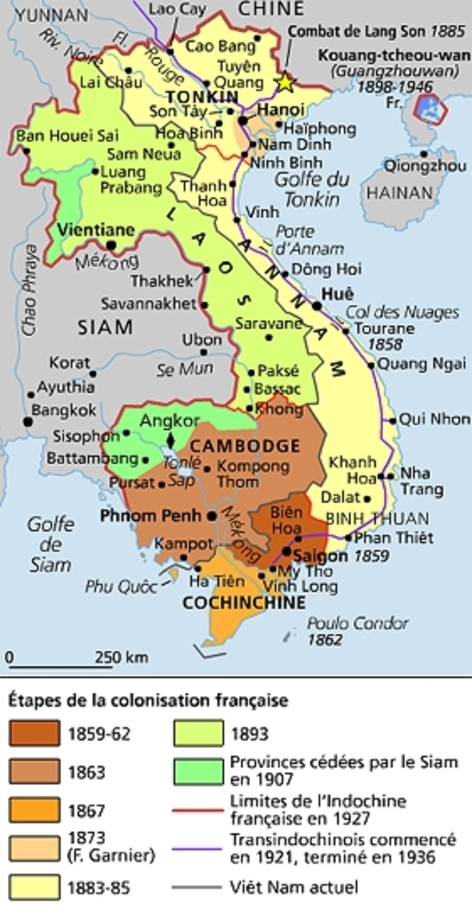
\includegraphics[width=0.5\linewidth]{img/1.1.union indochinoise.jpg}
    \caption{L'Union Indochinoise et ses étapes de la colonisation française}
    \label{fig:enter-label}
\end{figure}

« À partir du milieu du XIXe siècle, le royaume Dai Nam des Nguyen passe progressivement sous l’autorité française : après l’attaque du port de Tourane (actuellement Đa Nang) en 1858, Saigon est prise en 1859, le sud du pays devient une colonie française sous l’appellation de Cochinchine à partir de 1862 et le reste du pays, divisé en Tonkin et Annam, entre définitivement en 1884 dans l’Empire sous le régime du protectorat. La langue française étant la langue de l’administration coloniale, on forme des interprètes et autres auxiliaires indispensables à la marche des services. Il est logique de penser que les idées des Lumières ont dû s’introduire au Vietnam directement dans les fourgons du français. »\footnote{\cite{colon}}

L'un des principaux objectifs de cette colonisation était la Mission Civilisatrice. L'application de cette mission, quel que soit le territoire colonial, s'avérait complexe. Dans le cas spécifique du Vietnam et de l'Indochine dans son ensemble, cette mission revêtait une importance primordiale, symbolisant la transition des concepts scientifiques de l'orient vers l'occident.

« Plutôt « mission », d’amener ces civilisations inférieures au niveau de la civilisation française »
Des dichotomies telles que « Noir » et « Blanc », « sauvage » ou « barbare » et « civilisé », apparaissent alors comme autant de moyens mis en œuvre par le colonisateur pour justifier la domination des colonisés» \footnote{\cite{afri}}

Au commencement, au sein des colonies, des institutions intellectuelles et scientifiques coexistaient avec l'administration coloniale. Leur mission première était d'acquérir une compréhension approfondie des territoires colonisés, tout en contribuant aux buts plus larges de la colonisation. Toutefois, au fil du temps, des institutions universitaires autonomes ont émergé, poursuivant leurs propres objectifs de recherche indépendants. Les sociétés savantes constituent également une illustration de cette évolution. 
Cependant, \textit{que représente précisément la Société des études indochinoises ?}


%%%%%%Dans lequel la science ne fait pas partie importante, c'est pour ça que valoriser. Au XXe siècle, l'imprimerie s'est d'abord développée au Vietnam, Organisations et sociétés scientifiques savantes en générale


\section{Une première notion de la société savante}

La première société savante, qui reste la plus prestigieuse de ce statut est Académie des Inscriptions et Belles-Lettres - depuis 1652. Selon la définition de écrit par Régis Bertrand (Fédération historique de Florence) écrit dans le 1e Bulletin de liaision des sociétés savantes comme « une société qui produit et diffuse de la recherche, un groupe organisé dans un champ disciplinaire donné dont les adhérents ont pour objectifs de rendre compte de leurs travaux, d'améliorer la connaissance dans leurs domaines, d'assurer la formation et la recherche, de diffuser les résultats de leurs activités, de soutenir et de promouvoir leur discipline.»{\footnote{\cite{bum}}}

« la société de savoir pratique une attitude simplement cumulative des connaissances. Sonsouci n'est pas de mieux comprendre le monde qui l'entoure mais simplement d'engranger davantage de noms propres, de dates, de faits, et de descriptions. Jean Cluzel, secrétaire de l'Académie des sciences morales et politiques, évoque le rôle civilisateur de ces sociétés « dépositaires des anciennes traditions locales » {\footnote{\cite{alkd}}}

Il y a diverses définitions, cependant, les éléments généraux que nous retenons sont qu'une société savante se définit comme une organisation scientifique rassemblant des individus issus de diverses disciplines, tous animés par la volonté de développer la connaissance dans un domaine spécifique d'étude. L'adhésion à ces sociétés repose sur la volonté des membres de participer activement, cette participation étant soumise à l'approbation de leurs pairs. En plus de promouvoir la compréhension de l'objet de recherche, une société savante s'apparente à un institut intellectuel et comporte des éléments fondamentaux, notamment un conseil d'administration composé de présidents et de membres de l'association, un porte-parole scientifique, ainsi que diverses activités, telles que des séminaires et des cours en collaboration avec d'autres organisations scientifiques, généralement d'autres sociétés savantes.

Il est important de noter que les sociétés savantes fonctionnent selon un modèle horizontal, ce qui signifie qu'elles jouissent d'une certaine indépendance et ne sont pas directement subordonnées à une autorité académique supérieure. Elles établissent leurs propres normes et critères, et leur principale source de motivation réside dans la passion pour la recherche. Les considérations liées à la carrière et aux postes académiques ne sont pas prioritaires, la curiosité intellectuelle et la volonté d'explorer l'inconnu étant au premier plan. Dans le contexte des environnements coloniaux, caractérisés par des facteurs sociaux, géographiques et politiques inédits, de nouvelles disciplines scientifiques ont émergé, incitant les chercheurs à se tourner vers l'autoformation à partir des ressources scientifiques disponibles. Parallèlement, les sociétés savantes étaient interconnectées horizontalement, partageant une motivation commune visant à promouvoir une compréhension scientifique nouvelle.

Au sein de ces sociétés, une personne pouvait être membre de multiples associations, favorisant ainsi la diversification de la recherche et l'émergence d'approches interdisciplinaires au sein d'une même étude. Ces organisations soutiennent la recherche grâce à des infrastructures telles que des bibliothèques, des musées et des activités de recherche sociale, tout en favorisant la création d'un réseau social scientifique entre les chercheurs. L'objectif était de favoriser les échanges, la progression collective et d'apporter des éléments contribuant à une vision globale de l'objet de recherche, ce qui est illustré ici par le cas de la Société des Études Indochinoises (S.E.I) focalisée sur l'Indochine.

Un représentant du ministère de l’Éducation nationale a défini la société savante comme « un tissu associatif vivant » et « un des canaux de relations entre la recherche savante et la société civile ». \footnote{\cite{bbu}}

En effet, une société savante ne se limite pas uniquement aux activités de recherche scientifique internes, mais elle s'étend également vers l'extérieur en proposant diverses activités sociales. Cela inclut la tenue de séminaires, l'organisation d'expositions, ainsi que l'établissement de musées et de bibliothèques accessibles au public, favorisant ainsi la diffusion de la recherche scientifique auprès de la société en général. En résumé, une société savante entretient une étroite relation avec la société dans son ensemble.

« Tous ces courants donnent différentes catégories d’historiographie coloniale. On peut en distinguer grosso modo trois types. La première est constituée d’écrits de non-spécialistes, militaires et "coloniaux", travaux qui sont généralement des œuvres de commande? La seconde provient des travaux de propagandistes liés aux intérêts politiques et économiques de la colonisation, rédigeant et diffusant un savoir destiné à développer la fibre coloniale. Dans cette catégorie hybride, on trouve des auteurs appartenant au premier genre, mais aussi des savants, mobilisés pour la cause et capables de synthétiser une production hétéroclite. L'exemple le plus emblématique en est l'ouvrage paru en 1886 sous la direction d'Alfred Rambaud, professeur d’histoire à la Sorbonne: La France coloniale, Histoire, Géographie, Commerce”; après la préface de l'universitaire, les différents chapitres sont essentiellement confiés à des administrateurs et à des explorateurs. La même année voit la sortie d’un best-seller, Les Colonies françaises, rédigé sous les auspices d’un autre universitaire » .\footnote{\cites{marge05}}

Les sociétés savantes françaises ne se cantonnent pas uniquement à la France métropolitaine, elles élargissent leur champ d'action là où la science peut progresser et où de nombreuses découvertes restent à faire. L'exemple des sociétés savantes coloniales représente une forme de diffusion du savoir scientifique à l'échelle mondiale.

« Le troisième type d'histoire coloniale — que l’on pourrait qualifier de savante - se développe dans un cadre universitaire. S’appuyant sur le socle de publications produites par les catégories précédentes, mais surtout sur les sources passées au crible de la critique méthodique, ceux qui l’écrivent sont le pur produit du nouvel enseignement délivré à la Sorbonne. Rien, ni dans la méthode ni dans l’esprit général du travail, ne les distingue des autres travaux d'histoire. Leurs thèses sont rédigées selon les critères de rigueur scientifique de l’époque et ceux qui peinent à les satisfaire sont le plus souvent écartés de la carrière universitaire......Dulucq, Sophie, and Colette Zytnicki. » \footnote{\cites{marge05}}

La présence de ces organismes dans les colonies suscite également des interrogations quant à l'objectivité de leurs recherches. Dans cette étude, nous partons du principe que même si certains aspects de l'organisation des sociétés savantes sont étroitement liés à la politique, les études menées peuvent néanmoins être sujettes à des biais. Dans le cas de la Société des Études Indochinoises (S.E.I), les méthodes des humanités numériques seront utilisées en partie pour aborder cette question. 


\section{Société des études indochinoises}
« La crise ne fut, d’ailleurs, que passagères ; et quelques jours après la dissolution du comité ses anciens membres, réunis en séance extraordinaire, adoptaitent en principe sa reconstitution en une société libre appelée Société des Études Indo-chinoises »\footnote{\cite{soci}}

En quoi consiste exactement une société savante « libre » ? Comme l'indiquait le président George Dürrwell de la Société des Études Indochinoises dans son rapport adressé à Monsieur le Gouverneur général de l'Indochine le 30 septembre 1903, comme cité précédemment.

Après s'être « affranchie » du comité agricole et industriel de la Cochinchine, la nouvelle société, dotée de toutes les ressources précédentes mais arborant une nouvelle forme, est née. B.S.E.I a été fondée le 23 janvier 1883, immédiatement après la "suppression et la dissolution" du Comité agricole et industriel de la Cochinchine (1965-1883).

Si juste avant le Comité « fut placé sous la présidence du capital de frégate Fauque », « fut constituée avec des officiers de terre et de mer, soldats improvisés colons de la première heure »\footnote{\cite{a}} avec des missions bien définies dans le développement agricole de la colonie, l'organisation d'expositions, et bien sûr « dont les travaux insérés dans les bulletins du Comité prouvent qu’avec de la bonne volonté et de la persévérance, le Français est à la hauteur de toutes les situations » \footnote{\cite{a}}, et au cours de ces 18 années de développement, le Comité, dont il était l'un des «premiers ouvriers de la conquête dont les noms sont inscrits de droit au Livre d’Or de la Cochinchine » \footnote{\cite{soci}}. 

À ses débuts, le Comité agricole et industriel était un organe formel, peuplé en grande partie d'officiers de l'occupation française en Indochine. Son objectif initial était de superviser les expositions annuelles des produits locaux. La société fonctionnait selon des statuts rigides, avec des membres nommés par le gouverneur colonial.

Et au « 1er Octobre, le Comité comptait 107 membres et il était en rapport avec 17 sociétés savantes françaises ou étrangères. » \footnote{\cite{a}} . Cette phase prend fin, marquant ainsi la clôture de la première période historique et l'émergence d'un nouveau rôle en tant que revue continue du Bulletin de la Société des Études Indochinoises (B.S.E.I).

Toutefois, l'évolution politique et sociale de l'Indochine a provoqué une évolution majeure au sein de la S.E.I. En 1883, l'adoption de nouveaux statuts a marqué un tournant vers une structure plus démocratique. Désormais, les membres étaient cooptés plutôt que nommés, et la société bénéficiait d'une plus grande autonomie par rapport à l'administration coloniale à l'époque. 

Au fil du temps, la S.E.I. a élargi sa sphère d'intérêt pour englober une palette diversifiée de domaines, dans le statut de la société publiée année 1906 : 

« La S.E.I., continuant l'œuvre du Comité agricole et industriel, a pour objet l'étude de toutes les questions relatives tant à l'archéologie, aux arts, à l'ethnographie, et folklore, à la géograpbie, à l'histoire, à la philosophie, et aux religions, qu'à l'agri-culture, au commerce, à l'industrie et aux sciences de l'Indochine; elle s'intéresse aussi au rôle imparti à l'Indochine dans l'Extrême-Orient; elle conserve et transmet les monuments, archives et documents de toute nature, qu'européens qu'indigènes. »\footnote{\cite{bseik}}

La société a publié un Bulletin de ses travaux, entretenu des collections, participé à des expositions, commission et offert son soutien moral et intellectuel à diverses initiatives liées à ses domaines d'étude. Il conclut en notant que la société a publié un grand nombre d'articles au cours de ses 92 ans d'existence. Elle est constituée de plusieurs entités distinctes, notamment sa bibliothèque, sa scientifique et son musée.

Le Bureau de la société est composé d'un président, de deux vice-présidents, d'un secrétaire, d'un bibliothécaire, d'un trésorier et d'un conservateur de musée. Ces membres sont élus pour une durée d'un an et sont éligibles pour la réélection. Les élections pour le prochain Bureau ont lieu lors de l'Assemblée générale annuelle en décembre.

La société accueille un nombre illimité de membres, mais pour être admis, un candidat doit être parrainé par deux autres membres de l'association et doit obtenir les votes favorables de 2/3 des membres présents. Les membres peuvent également être révoqués de leur statut dans certaines circonstances, telles que leur démission volontaire, une absence prolongée ou s'ils sont exclus par les autres membres de l'association.

Il existe trois principales catégories de membres au sein de la S.E.I : les membres honoraires, qui sont désignés par le Bureau et qui peuvent être des étrangers, des fonctionnaires ou des individus ayant contribué de manière significative à la recherche sur l'Indochine ; les membres titulaires, qui résident en Indochine ; et les membres correspondants, qui résident à l'extérieur de la région.

Selon Martine François dans son article de \textit{Les sociétés savantes et l’histoire des voyages et des explorations} :
« Nous pouvons distinguer trois types de sociétés susceptibles d’avoir conservé des fonds intéressant les voyages, tout d’abord, celles créées spécialement pour étudier un pays, un continent, ce qui légitime la constitution de ces fonds."\footnote{\cite{ak}}
« Les sociétés consacrées à des pays ou à des continents Dès le milieu du XIXe siècle des sociétés savantes furent créées dans les territoires nouvellement colonisés comme la Société d’histoire et d’archéologie de Constantine, la Société historique algérienne, l’Académie d’Hippone, la Société des études indochinoises, l’Institut de Carthage, la Société des sciences, lettres et arts de la Réunion ou l’Académie malgache. Ces sociétés ont été les premières à étudier l’histoire et l’archéologie de ces pays nouvellement découverts. » \footnote{\cite{ak}}

En réalité, la Société des études indochinoises (S.E.I) est réputée pour être une société érudite dédiée à l'étude de pays ou de continents spécifiques. La Société des Études Indochinoises n'est pas la seule société savante coloniale française. On peut mentionner d'autres organisations de ce type, notamment aux colonies françaises : 

\begin{itemize}
    \item Société royale des Artes et des sciences de l’Ile Maurice
    \item Société d’agriculture d’Alger
    \item Société géographie et d’archéologie de la province d’Oran
    \item Société des sciences et art de la Réunion, ect.
\end{itemize}

En Indochine : 
\begin{itemize}
    \item Société médico-chirurgicale de l'Indochine \footnote{\cite{al}}
    \item Société médicale de Saigon – SAIGON\footnote{\cite{ab}}
    \item Société de géographie d'Hanoï (1921-)
    \item L'école française d'Extrême-orient
    \item Association des Amis du Vieux Huê
\end{itemize}

En 1933, lors de la célébration du cinquantième anniversaire de sa fondation, la Société des études indochinoises (S.E.I) avait déjà émis un total de 388 numéros de publication. Cela indique qu'en comparaison avec l'ensemble des journaux dont nous disposons des données pour notre corpus sera 1342 articles, la période qui est suivie n'a duré que 42 années. Toutefois, il est remarquable que leur productivité ait considérablement augmenté par la suite (1933-1975), atteignant finalement un total de 954 numéros de publications.

En 1893, la société a élargi ses horizons en introduisant le tourisme au sein de ses activités, sous l'impulsion de M. Commençait. Cependant, cette initiative a failli causer sa perte en 1925 lorsque le Bulletin a fusionné avec la Revue du Tourisme. Heureusement, la société a réussi à rebondir l'année suivante, en 1926.

Le logement en premier temps a toujours été un défi pour la société. En 1887, elle a été brusquement expulsée de ses locaux et a déménagé précipitamment, stockant sa bibliothèque, ses archives et ses meubles dans un compartiment de case malabare. Elle a ensuite loué un immeuble à colonel Rheinart pour 50 dollars par mois en 1887, puis a élu domicile à la société Philharmonique en 1891. En 1897, elle a emménagé au 16 rue Lagrandière, un immeuble appartenant à l'Évêché, où elle est restée pendant 20 ans. Enfin, elle a trouvé un emplacement stable au 12 Boulevard Norodom, dans un immeuble chrétien, pour 10 000 francs.\footnote{\cite{societe}}

L'un des moments forts de la société a été la contribution de M. Mercier Beauné en 1893, lorsqu'il a présenté des pierres préhistoriques gravées trouvées à Tay Ninh. En février 1897, un "air anthropologique" est né grâce à M. James, rédacteur en chef du Courrier de Saigon, qui a partagé des objets étranges parmi les membres, dont des armes, des colliers, des bijoux en os, en pierre et en cuivre, ainsi que des fragments de squelettes. Il a promis de céder une partie de sa collection à la société. Le général de Beylié a également contribué en fournissant d'importants moulages de vieilles pierres artistiques d'Angkor au musée\footnote{\cite{societe}}. 

Ces pionniers experts ont joué un rôle fondamental en traçant les premières lignes directrices de la recherche au sein de la Société des Études Indochinoises, marquant ainsi une transition significative dans leurs domains de recherche.

À une époque où l'Indochine était encore largement associée à l'agriculture et à l'exploitation des ressources naturelles, ces experts ont apporté une perspective nouvelle en se tournant vers l'archéologie et la préhistoire. Leur vision audacieuse a ouvert de nouvelles avenues pour la compréhension de l'histoire ancienne de la région, jetant ainsi les bases de la recherche archéologique et préhistorique qui allait suivre.

Le fonctionnement de la société a été un défi constant en raison de ses préoccupations scientifiques et philosophiques, conjuguées à des besoins matériels : 

« Les plus hautes préoccupations scientifiques et philosophiques y ont fait bon ménage avec des soucis très matériels: le local, le musée, les cotisations, les subventions, l'argent, pour tout dire en un mot, nécessaire non pas à rémunérer des travailleurs tous bénévoles, mais à payer le loyer, le personnel, l'éclairage, l'imprimeur, achats de livres, les abonnements aux revues, les timbres-poste et le papier de la correspondance parfois volumineuse qu'on échange avec l'Administration, avec les sociétés savantes d'outremer, avec les membres de la métropole... »{\footnote{\cite{societe}}}

Le 2 septembre 1945, à la place Ba Dinh de Hanoï, Ho Chi Minh proclama la création de la République démocratique et indépendante du Vietnam. La guerre de résistance commençait dans le Sud, également connue sous le nom de Nam Bô kháng chiên, fut un conflit armé qui a eu lieu après la Seconde Guerre mondiale. Il impliqua les Britanniques, les Indiens, une force opérationnelle française ainsi que les troupes japonaises du Groupe d'armées expéditionnaire japonais du Sud, qui se sont trouvés en opposition avec le mouvement vietnamien communiste, le Viêt Minh, dans le but de déterminer le contrôle du pays. 
Pour la toute première fois, notre société s'est retrouvée confrontée à des événements majeurs susceptibles de mettre en péril son existence. En effet, c'est la première fois que, en ouvrant les premières pages du Bulletin, nous avons été accueillis par un avertissement évoquant la situation politique actuelle. Dans le rapport moral du président de l'organisation, nous avons également constaté une préparation résolue à affronter d'éventuelles dérives. 

« L’année qui vient d’achever a été marqué par la volonté persistante de votre Comité de maintenir l’activité de la Société des études indochinoises dans la voie qu’elle s’est tracée dès le début de la guerre qui consiste à poursuivre sans défaillance l’œuvre entreprise il y a plus de soixante ans. »\footnote{\cite{moral1}}
Et aussi : 
« Quelle que soit l’incertitude du lendemain, une tache immense est offerte aux hommes de bonne volonté. Même si notre bulletin devait renoncer à paraitre, notre effort n’en serait pas ralenti et nous ne cesserions de susciter des recherches et d’accueillir, pour une résurrection très proche, le fruit de ces travaux »\footnote{\cite{moral1}}

Deux années se sont écoulées, mais la situation n'a montré aucune amélioration. En 1947, le président M. Berland a présenté un autre Rapport moral, marquant ainsi une nouvelle étape dans l'évolution de notre société. Cette fois-ci, des changements significatifs ont été apportés à notre statut, principalement en ce qui concerne les cotisations des membres. De plus, une recommandation audacieuse a été formulée : l'introduction de deux nouveaux titres inédits, celui de « membre bienfaiteur » pour ceux faisant un don de 200 dollars, et celui de « membre à vie" pour ceux qui contribuent à hauteur de 500 dollars en faveur de la société. 
« Au 9 Mars 1945, le nombre de nos sociétaires s’élevait à 507. Au 30 juin 1946, nous nous retrouvions 150. Cette chute verticale était imputable, pour une large part, aux rapatriements massifs et aux bouleversements introduits dans la vie de chacun »\footnote{\cite{moral}}
et aussi plus précisément dans l'article du projet de modification :
« Le comité arrête le détail des modifications aux statuts à soumettre à l’Assemblé Générale du 19 janvier, en ce qui concerne notamment le nouveau montant des cotisations, ainsi que l’adaptation du libellé de divers articles, relatifs à l’organisation nouvelle de l’Indochine. »\footnote{\cite{change}}


En ce qui concerne la présidence de la société, elle a été incarnée par des figures notables, dont :

\begin{itemize}
    \item \textbf{D. Mougeot (1883-1904)}, qui a été à la tête de la société pendant une période cruciale de son développement.
    \item \textbf{M. Dejean de la Bâtie (1904-1906)}, qui a poursuivi le travail de son prédécesseur.
    \item \textbf{M. Tanan et M. Durrwell}, qui ont partagé la présidence pendant une impressionnante période de 14 ans, marquée par des réalisations significatives.
    \item R\textbf{aphael Barquisseau (1933-)}, qui a apporté sa contribution à la société dans une période d'importants changements historiques.
   \textbf{ H. Berland (-1949)} qui a soutenu la société la période marquée par le changement de statut de la société
    \item \textbf{MM. Gayet Georges (1949-1950)} et Doan Quang Tuan (1950-1952), qui ont dirigé la société dans une période charnière.
    \item Enfin, le dernier président de la société, \textbf{M. Joseph Boquet (1952-1975)}, a exercé ses fonctions avec dévouement pendant 23 ans, marquant ainsi une ère importante de l'histoire de la société. Il a été épaulé par le vice-président Truong Vinh Tong.
\end{itemize}

Ces présidents, chacun à leur manière, ont contribué à l'épanouissement et à la renommée de la Société des Études Indochinoises, faisant d'elle une organisation emblématique de l'étude et de la préservation du patrimoine indochinois.


\subsection{\textbf{Activités de la société
}
}
La société des études indochinoises a joué un rôle essentiel dans un éventail diversifié d'activités et d'événements marquants au fil de son histoire, en Indochine et à l'international. Parmi les moments clés de son engagement, on peut citer :

\begin{itemize}
    \item Exposition de 1900 et Exposition coloniale de 1931 : La société a pris part à ces expositions prestigieuses, contribuant ainsi à mettre en lumière la richesse culturelle de l'Indochine.
    \item Communication au Congrès des Sociétés Savantes (1891) : Une communication significative sur les ressources naturelles indochinoises a été présentée par J. Schroeder, illustrant l'expertise de la société dans ce domaine.
    \item Congrès International d'Histoire des Relations Culturelles entre l'Occident et l'Orient à Tokyo (1957) : Un événement d'envergure internationale auquel la société a participé activement, favorisant ainsi les échanges culturels.
    \item Exposition d'Arts et d'Archéologie du Vietnam à Washington (1960) : La société a contribué à cette exposition majeure qui a permis de partager la richesse artistique et archéologique du Vietnam.
    \item Exposition d'Art Français au Japon à Tokyo (1961) : Une autre manifestation témoignant de l'influence culturelle et de la coopération internationale soutenue par la société.
    \item Conférence Régionale Asiatique sur l'Éducation des Adultes (1951) : La société a activement participé à cette conférence d'importance régionale, mettant en avant son engagement dans des domaines divers, dont l'éducation.
\end{itemize}

\subsection{{Mussée Blanchard de la brosse
}}

Un des éléments importants dans l'identité de la société savante indochinoise est également le rôle central joué par la S.E.I. dans la création du Musée archéologique et artistique de Saigon (Musée Blanchard de la brosse, le nom d'un diplomate et gouverneur colonial français). Initialement, l'idée de créer un musée n'était pas à l'ordre du jour, mais au fil du temps, la société a progressivement investi dans ce projet, contribuant à rassembler des objets et des spécimens d'origine indochinoise pour ce qui allait devenir une institution culturelle significative.

Depuis l'année 1897 a été témoin d'un moment décisif lorsque Ludovic Jammes, membre éminent de la société, a émis la proposition audacieuse d'une expédition dans les environs de Pursat, au Cambodge. Son objectif : collecter des objets préhistoriques. Le succès de cette expédition a rapidement incité la société à créer une commission dédiée à l'étude et à la mise en place d'un musée ouvert au grand public. La Société des Études Indochinoises a dû surmonter de nombreux défis au fil de son histoire, des difficultés financières et des conséquences de la Première Guerre mondiale aux promesses non tenues pour la construction d'un musée du gouvernement, et ce, jusqu'au 14 août 1929, marquant une date mémorable, le musée archéologique et artistique de Saigon a été officiellement inauguré lors d'une cérémonie imposante. Cela a dû être une décision importante, car la fondation a dépensé jusqu'à 45 000 piastres pour acheter la collection de M. Holbé comme plate-forme d'exposition pour le musée, sachant que la cotisation de l'association n'était que d'1 piastre par mois et que l'association ne disposait que d'environ 200 personnes. Cette décision fit alors grand bruit dans la presse indochinoise à propos d'un musée Blanchard de la brosse nouvellement né.  

« Au temps où il arrivait à Saïgon, mourait dans cette ville un ancien pharmacien de la marine, le docteur Holbé qui, au cours d'une longue carrière passée toute entière dans nos parages, avait réuni avec infiniment de science, d'admirables pièces d'art chinois, japonais, coréen, thibétain, khmer, siamois, javanais et indou. »\footnote{\cite{collection}}

Peu de temps après, il a ouvert ses portes au grand public, offrant ainsi à tous un accès aux richesses culturelles et historiques de l'Indochine :
« M. Bouchot, conservateur du musée Blanchard de
la Brosse, rend compte que le nombre des visiteurs du musée pour le mois de février 1929 s’est élevé à 10.458 contre 10 883 en janvier. » Dont 3932 Européens et 6526 indigènes.\footnote{\cite{bouchot}}

La société a continué à une participation actif dans la gestion du musée, contribuant à son développement et à l'enrichissement de ses collections. Les présidents de la société ont joué un rôle essentiel dans cette entreprise, en mobilisant des ressources et en garantissant l'engagement continu de la société envers le musée. Un personnage important est Jean Bouchot(1929-1932) comme directeur et Louis Marius Malleret les conservateurs du musée pendant la période 1935-1949. Pourtant, du 1956 à 1979, par rapport au contexte historique le musée devient musée national du Viêt Nam à Saïgon.

Lorsqu'il s'agit d'évoquer le succès et la reconnaissance de la société au sein de la communauté scientifique, cela ne peut tout simplement citer le message de félicitation de l’École français d’Extrême-Orient de Louis Malleret : 
« La société des études Indochinoises héritière de la tradition léguée par l’ancien Comité agricole et industriel de la Cochinchine, l’avait précédé depuis 1883 dans la voie de travaux de recherches. Des officiers de marine et des érudits vietnamiens s’étaient associés très tôt pour accomplir un premier inventaire de connaissance et susciter un mouvement de découvertes dans le domaine de l’exploration géographique, des investigations archéologiques et des études philologiques. »\footnote{\cite{feli}}
et aussi
 « la société a connu trois guerres et s’est invariablement remise à la tache avec une nouvelle ardeur. »
« Depuis les temps ont passé, les générations se succèdent et les recherches scientifiques sont devenues plus pénétrantes et plus sûres de leurs méthodes et de leurs résultats. »\footnote{\cite{feli}}

Dans la dernière revue publiée en 1975, la société elle-même a également consolidé sa position dans le domaine des études indochinoises, comme en témoigne le comité de rédaction écrivait :
« Doyenne des sociétés savantes en Indochine. Créatrice du musée Blanchard de Saïgon, qu'elle administrait. La société d'études indochinoises, poursuit l'œuvre du Comité agricole et industriel créé en 1865. Elle compte dès 1883, 300 membres actifs européens et indochinois. Elle est en relation avec 38 sociétés savantes et universités françaises. »\footnote{\cite{fin}}
Ceci est également noté dans la page de définition de l'organisation pour S.E.I dans le site web de la Comité des travaux historiques et scientifiques.

\textbf{La bibliothèque de la société des études indochinoises
}
La Bibliothèque de la Société des études indochinoises occupe une place de premier plan dans le paysage intellectuel de l'Indochine. Depuis ses débuts, elle a été le réceptacle d'une multitude de dons de livres, chacun d'une valeur inestimable et provenant de sources diverses. Les collections de la bibliothèque sont riches et variées, reflétant la diversité des intérêts et des domaines de recherche de ses membres.

L'évolution de la Bibliothèque de la Société des Études Indochinoises est aussi un aspect à remarquer. La bibliothèque a été constituée par des dons de provenance variée, ce qui a donné à sa collection un caractère hétérogène. Elle s'est d'abord concentrée sur des domaines tels que l'agriculture tropicale, la zootechnie, les produits industriels et les sciences naturelles. Avec le temps, la bibliothèque s'est élargie pour englober des domaines d'études sur l'Indochine et l'Extrême-Orient.

L'héritage de la bibliothèque remonte aux premiers catalogues du Comité agricole et industriel, qui comprenaient des sections consacrées à l'agriculture tropicale. Au fil du temps, la bibliothèque s'est élargie pour englober des sections dédiées aux Beaux-Arts, à l'archéologie, à l'histoire, à la physique et aux sciences naturelles. Les collections de périodiques et d'ouvrages rares ont également trouvé leur place au sein de ses rayons.

La diversité culturelle de l'Indochine se reflète également dans les collections de la bibliothèque, qui abritent plusieurs fonds locaux, notamment chinois, khmer, laotien et siamois. Les estampes, les photographies et les manuscrits des membres de la société, tels que A. Adhémard Leclère, Silvestre, Charles Lemire, ajoutent une dimension précieuse à ces collections.

Au cours de son histoire, à notre connaissance, la bibliothèque a entrepris plusieurs réorganisations en 1927, 1930 et 1933, afin de mieux répondre aux besoins de ses membres et de garantir un accès optimal à ses précieuses ressources. Elle a également procédé à des achats urgents en réponse aux demandes spécifiques de ses membres, démontrant ainsi son engagement envers la recherche et la diffusion des connaissances.

« Mais, quoi qu'il en soit de ses défauts, elle n'en est pas moins l’un des centres de documentations les plus précieux que l'on possède en Indochine, sur les questions qui intéressent ce pays et l'Extrême-Orient La Bibliothèque de la Société des Etudes Indochinoises pourrait, dans une modeste mesure, jouer en Cochinchine, le rôle que détient au Tonkin la Bibliothèque de l'École française d’Extrême-Orient. Il lui appartient, en effet, de spécialiser son objet dans la réunion de tous les ouvrages qui se rapportent à l'Indochine et aux pays voisins. » \footnote{\cite{bilo}}. Parmi les ouvrages importants qui composent ses collections, on peut citer des œuvres historiques et scientifiques telles que :

\textit{Le Catéchisme en latin et en quôc ngu de P. Alexandre de Rhodes} (1651), \textit{Les Divers Voyages et Missions du P. Alexandre de Rhodes en la Chine et autres Royaumes de l'Orient} (1654), \textit{Le Recueil de plusieurs Relations et traités singuliers et curieux de J. B. Tavernier} (1679), \textit{La Relation des Missions et des Voyages des Évêques vicaires apostoliques ès années 1673, 1673, 1674 et 1675} (1680), \textit{Le Journal du Voyage de Siam fait en 1685 et 1686 par l'abbé de Choisy} (1687), \textit{Le Nouveau Voyage autour du Monde de Le Gentil de la Barbinais} (1728), ect. aujourd'hui considérés comme des trésors inestimables.\footnote{\cite{bilo}}

En matière de préservation et de diffusion du savoir, la Bibliothèque de la Société des Études Indochinoises est à juste titre reconnue en tant qu'institution éminente, établissant ainsi une égalité remarquable avec la Bibliothèque de l'École française d'Extrême-Orient. Ensemble, ces deux institutions contribuent de manière significative à l'enrichissement du patrimoine intellectuel de l'Indochine et à la compréhension approfondie de la région et de ses multiples facettes.


%Les membres sont membre de plusieurs sociétés savantes différentes."

%Discours politique, eurocentrique, discours colonial
%Dans le status de la société, la première fois apparait
%\textit{"Toute discussion politique ou religieuse est interdite"
%Ce changement remarque

\section{Le Bulletin de la société des études indochinoises}

Parmi les revues scientifiques les plus influentes dans le contexte de la vie intellectuelle en Indochine au début du XXe siècle, en plus des publications de l'École française d'Extrême-Orient (EFEO), du Bulletin des amis du vieux Hué (BAVH), de la revue Indochina, et de Littérature et Histoire, il est incontournable de mentionner le Bulletin de la Société des Études Indochinoises (B.S.E.I). Cette revue a vu le jour pour la première fois le 23 janvier 1883, et dès son premier numéro, à l'article 25, on pouvait lire :

« Le Bulletin est ouvert à la publication de tous les travaux susceptibles de diffuser la connaissance des diverses parties de l’Indochine, de leur géographie, de leur population, ressources, besoin, langues, ect. Il contient, de plus, les décisions de l'autorité concernant son œuvre, les-rendus des séances, des extraits ou des résumés des travaux étrangers intéressant les comptes régions indochinoises et un bulletin bibliographique, analytique autant que possible. »

Le nom du Bulletin est en étroite corrélation avec l'association SEI, car son objectif premier est la diffusion des connaissances scientifiques liées à l'Indochine. De plus, il joue également le rôle d'organe de communication de l'association, favorisant ainsi les échanges avec d'autres sociétés savantes en France et à l'international. Au cours de ses 92 années d'existence, la revue s'est engagée à évoluer bien au-delà de ses débuts modestes.

Dans un premier temps, le comité de rédaction du journal a envisagé la création d'un magazine mensuel de seulement 16 pages par numéro. Cependant, cette idée a rapidement évolué vers la publication d'une revue de 50 pages tous les trois mois, ce qui a été jugé plus réaliste. Le premier numéro ne contenait que deux rapports, et les numéros suivants maintenaient une moyenne d'environ 50 pages, comprenant des comptes rendus de la société et des articles sur l'organisation de l'association. Entre 1886 et 1887, la revue ne produisait que deux numéros par an (au lieu des quatre prévus), mais ceux-ci comptaient environ 70 pages chacun.

À partir du dernier numéro de l'ancienne série en 1919, la revue a progressivement augmenté sa pagination pour atteindre environ 200 pages par numéro. Les numéros de la nouvelle série ont même dépassé les 500 pages (comme le numéro 4 en 1953). Cette évolution témoigne de la croissance des intérêts et de l'expérience des auteurs, ainsi que de l'émergence d'une équipe d'auteurs de plus en plus solide, tant en termes de qualité que de quantité.

Il est important de noter que le B.S.E.I ne fixe pas de limites strictes en ce qui concerne le nombre de pages par numéro. La longueur des numéros varie en fonction de la diversité des genres et des sujets abordés. L'Indochine demeure un terrain de découverte scientifique, une jeune colonie, offrant ainsi aux auteurs et intellectuels éloignés de la France l'opportunité d'explorer et de comprendre cette région. Ils y trouvent un champ intellectuel stimulant et sérieux, tout aussi captivant que celui de leur pays d'origine.

De nombreux auteurs vietnamiens ont été éduqués dans le système occidental et ont fréquenté les écoles françaises dès leur plus jeune âge. Bien qu'ils parlent vietnamien, leur esprit scientifique et leur pensée théorique sont aussi développés que ceux de leurs homologues européens. Ils ont adopté des approches rationnelles et se sont rapidement intégrés à la vie intellectuelle en émergence. La diversité des contenus est une caractéristique majeure de la revue, et les exemples mentionnés ci-dessus ne représentent qu'une infime partie de la richesse du contenu global du journal.

\textbf{Thèmes de la religion} : Le bouddhisme en général par D. Migot (1946), Quelle est la religion des Annamites ? par L. James (1895), La religion les montagnards du Haut-Donnai par J. Dourne (1949), Contribution à l'étude du Culte des génies tutélaires ou Neak Ta chez les Cambodgiens du Sud par A. Souyris Rolland (1951) .. 

\textbf{Éducation} : L’enseignement en Cochinchine par G. Taboulet (1942), De l’enseignement du français en Indochine par J. B de Saint Michel, Le français et le vietnamien dans l’enseignement au Vietnam par Doan Quan Tan (1954) de la chimie Etudes des minéraux lourds de quelques sables littoraux par Hoang Ngoc Can (1964)

\textbf{L'ethnologie} : Le peuple en Asie par Teilhard de Chardin (1955), Études anthropologiques par P. Huard (1947), Notes d'ethnographie Cochinchinoise par C. Richard (1927), etc. 

\textbf{Géographie} : Les origines de Hanoi par G. Azambre (1958), Les mobiliers préhistoriques de l'abri sous roche de Tam Pong (Haute Laos) par E. Saurin (1966) 
Folklore laotien : Xine-Xay, par Thao NHOUY (1934) 

\textbf{Littérature vietnamienne} : Chinh phu nam khuc (Femme de guerrier) par Doan Thi Diem traduction Huynh Khac Dung (1955)… 

\textbf{Médecine} : De la diffusion de médecine européenne en Cochinchine par Péralle (1895), L'art de guérir chez les Annamites par L. James (1896), Histoire de l'acupuncture chinoise par P. Huard et Wong (1957)... 

\textbf{Les langues} : Petit vocabulaire laotien par J. Taupin (1892), Essaie sur l'origine de la langue  Annamite par G. Janneau (1883) ou La forme politesse en Javanais moderne par C. Damais (1950) 

Aussi nombreux articles sur \textbf{l’archéologie}, \textbf{l’histoire moderne}, \textbf{l'agriculture}, \textbf{la botanique}, \textbf{l'industrie}, \textbf{l'art}, \textbf{l'architecture}..
La revue B.S.E.I. (Bulletin de la Société des Études Indochinoises) se présente comme un véritable guide de l'Indochine, offrant une palette thématique d'une richesse étonnante. Cependant, il est révélateur de noter que, en 1923, la revue a connu de nombreuses difficultés pour assurer sa publication régulière.

Ces obstacles étaient principalement d'ordre économique, ce qui a conduit à des interruptions dans la publication en 1920, 1921, 1922, 1924 et 1925. Cependant, il est important de noter que ces interruptions dans la publication n'ont pas interrompu les réunions mensuelles de l'association. Les procès-verbaux de ces réunions ont été intégralement réédités pour que les membres puissent toujours accéder à ces informations, avec des numéros spéciaux en 1923 et 1926. Cela peut s'expliquer par le fait que la plupart des lecteurs de la revue sont des membres inscrits, et la responsabilité de l'éditeur peut inclure la réédition d'informations sur la société.

La revue B.S.E.I. ne se limite pas à être uniquement une publication scientifique, il sert également de lieu de diffusion pour toutes les informations liées à la société. Il fonctionne en quelque sorte comme un canal d'informations sur la société savante et les travaux de recherche scientifique de ses membres. Selon les statuts de l'association en 1883, la revue était distribuée gratuitement aux membres, tandis qu'une cotisation était due par les membres titulaires et correspondants. Cette cotisation était fixée à deux piastres par mois, payables trimestriellement et à l'avance, mais elle était réduite à 1 piastre par mois lorsque le nombre de membres titulaires dépassait cent. Les membres honoraires n'avaient pas de cotisation à payer.

Au cours de ses 92 années de développement, B.S.E.I. a connu deux périodes distinctes : l'ancienne série de 1883 à 1920, intitulée "Bulletin de la Société des Études Indochinoises de Saigon", puis la nouvelle série de 1926 à 1975, sous le nom de "Bulletin de la Société des Études Indochinoises". Durant cette période, les numéros étaient regroupés par année, avec un système de classement basé sur les "Tombe", chaque année comptant quatre numéros correspondant à chaque saison. Au total, B.S.E.I. compte 135 numéros au total, mais ces numéros ne sont pas numérotés séquentiellement, mais plutôt par année.

L'origine de B.S.E.I. remonte à son prédécesseur, le Bulletin du Comité, qui était principalement administratif. En 1883, il a évolué pour devenir un véritable bulletin d'études scientifiques. Présenter la revue B.S.E.I. est une tâche complexe, car elle est peu connue dans les résultats de recherche classiques, mais elle est considérée par les experts scientifiques comme une revue scientifique précieuse en tant que porte-parole de la plus ancienne société savante d'Indochine, non pas en tant que successeur d'une autre revue savante, mais pour ses propres mérites. En 1896, pour la première fois, les statuts de la société ont énoncé :

\begin{figure}[H] %[!ht]
    \centering
    
\includegraphics[width=1\linewidth]{img/tout.PNG}
    \caption{Statut de la société en 1896}
    \label{fig:enter-label}
\end{figure}

Une simple phrase, isolée de l'article Ier de ce texte, suggère que la société savante a peut-être réussi à évoluer au-delà de sa forme initiale de comité placé sous le contrôle du gouvernement colonial. Cette observation invite à prendre position en dehors des contextes politiques et religieux.

Cela étant dit, il existe un paradoxe notable, car même dans la plupart des numéros de la société pendant cette période, la liste des membres inclut toujours des personnalités telles que M. Le Gouverneur Général de l'Indochine en tant que président d'honneur, aux côtés de M. Le Lieutenant-gouverneur et du Général commandant la brigade de Cochinchine, entre autres, en qualité de vice-présidents d'honneur. De nombreux membres de la société étaient des individus travaillant au sein du gouvernement colonial, des fonctionnaires intellectuels dont les carrières étaient étroitement liées à la situation politique de l'Indochine à l'époque.

Cependant, malgré leur rôle dans le gouvernement colonial, ces individus étaient animés par une curiosité intellectuelle et un engagement envers la science qui les poussaient à s'engager dans des débats non politiques et non religieux, mais centrés uniquement sur les questions de recherche liées à l'Indochine.

Le B.S.E.I a hérité de son prédécesseur initialement un axe sur la mission d'apprentissage agricole et industriel, a progressivement élargi son champ d'intérêt pour englober tous les domaines liés à l'Indochine, avec une orientation claire vers la diffusion du savoir. En 1883, les trois premiers numéros du journal étaient centrés sur des sujets tels que "les grains jaunes du riz", "les cultures expérimentales", "les comptes rendus sur les courants terrestres", etc. Cependant, au fil du temps, la revue a évolué et diversifié ses thématiques, comme nous le démontrerons dans les analyses quantitatives ultérieures.

En raison du fait que notre compréhension actuelle de cette revue est encore en cours de développement, il existe très peu de sources extérieures d'information sur le B.S.E.I, à l'exception de ses propres publications. Les auteurs des articles publiés dans le B.S.E.I sont à la fois français et vietnamiens, et ils collaborent pour enrichir les connaissances. Parmi les Français qui ont contribué de manière significative, on peut citer : \textbf{André Baudrit, Jean Bouchot, Pierre Brocheux, Arthur Chéon, Pierre Daudin, George Dürrwell, Maurice Durand, Louis Ricard, Louis Malleret, Geogrette Naudin ; Henri Marchal}… 

\textbf{Henri Marchal }: \textit{Le chanteur d'Angkor Wat} (1934), \textit{Le temple de Banteay Srei} (1936), \textit{Notes sur Birmanie} (1950), \textit{Les travaux de la conservation d'Angkor} (1953), \textit{Notes sur un théâtre à l'ombres à Siem Reap} (1958), L\textit{Le Naga dans l'art khmer} (1937)… 

\textbf{Pierre Daudin} avec \textit{Vue ensemble sur la sculpture et la modelage en Chine durant vingt siècles} (traduction en 1936), \textit{Note sur un cachet en ou découvert en Annam} (1936), \textit{Sigillographie sino-annamite}(1937), \textit{Deux mandarins militaires de Thieu- Tri : Le Sam et Trieu Tan} (1943), \textit{Un Japonais à la Cours des T'ang, Gouverneur et protectorat d'Annam }(1965)… 

 \textbf{George Dürrwell} avec \textit{Les colonies militaires dans la Basse-Cochinchine} (1998), L\textit{e jeu en Cochinchine} (1901), \textit{La famille annamite et les cultes des ancêtres} (1908), \textit{La commune annamite} (1905),\textit{ Une visite à Ong-Yem : Les champs d'essai et la colonie pénitentiaire} (1909)… 

\textbf{Arthur Chéon} a traduit \textit{Des langues monosyllabiques du Sud de l'Asie} (K. Himly) (1886), \textit{Histoire de La-to ; La vase qui parle} (1889) ou \textit{Notes sur l'origine des chants populaires annamites} (1989), \textit{Notes sur la chanson cambodgienne} (1890) 

\textbf{Maurice Durand} : \textit{L'avenir des études vietnamiens }(1953), \textit{Chants des pêcheurs de Truong-Dong} (culte de la baleine) (numéro 2, 1953), \textit{Quelques éléments sur l'univers moral des Vietnamiens} (1952), A\textit{lexandre de Rhodes} (1957), \textit{Les impressionnants en vietnamien} (1961), L\textit{a Science au Vietnam} (avec P.Huard)( 1963) 

Selon nos observations, au fil du temps, le nombre d'auteurs vietnamiens participant à la rédaction de journaux augmente, les noms typiques incluent des intellectuels célèbres : 
Nguyen The Anh est spécialisé dans la rédaction d'articles historiques. 

\textbf{Vuong Hong Sen} avec des articles sur la culture chinoise \textit{La pagode de l'Empereur}(1950),\textit{ Le Jade à Dakao} (1950), \textit{Les pot à envoûtement, ancêtres des flacons à parfum moderne} (1949) 

\textbf{Nghiem Toan} et \textbf{Louis Ricard}, co-traducteur de contes chinois, peuvent citer \textit{Histoire du Ou Pao An} (1958). Leurs traductions sont d'une grande qualité, au point qu'aujourd'hui \textit{Les trois royaumes} (publié sur B.S.E.I de 1960 à 1963), le premier des Quatre livres extraordinaires de la littérature classique chinoise, sa traduction est rééditée aux éditions Flammarion depuis 2009 jusqu'à aujourd'hui. 

\textbf{Tran Van Khe} introduit \textit{Mise au point de l'étude sur la musique sino-vietnamienne et les chants populaires du Viêt-Nam} (1959) ou \textit{Place de la musique dans les classes populaires au Vietnam} (1959) 

Les deux frères \textbf{Truong Vinh Ky} et \textbf{Truong Vinh Tong}, dont \textbf{Petrus Ky}, participèrent dès les premiers jours au Bulletin du Comité et poursuivirent leurs écrits au B.S.E.I avec des articles sur \textit{L'Ecriture en Annam} (1888) ; \textit{Chuyen doi xua : Contes d'autres fois : Le genre qui veut intimider son beau-père} ; \textit{Le renard et le tigre} traduits par \textbf{Truong Vinh Tong} (1932), ect.
Toutes ces histoires ont été traduites en français par Truong Vinh Tong, son jeune frère, et le texte est présenté de manière bilingue. Il est intéressant de noter que, à l'exception de Truong Vinh Ky, les autres auteurs sont tous apparus après 1950, ce qui témoigne clairement de l'émergence d'une nouvelle génération d'intellectuels vietnamiens participant à la rédaction de la revue.

Dans le numéro de 1967, quelque chose de remarquable s'est produit pour la première fois dans B.S.E.I : des titres d'articles et des annotations bilingues en vietnamien avec des accents complets ont fait leur apparition. Cette évolution linguistique montre une ouverture vers une audience vietnamienne plus large. Même dans le numéro de 1972, il y avait un article consacré à la poésie de Han Mac Tu qui s'étendait sur 108 pages. Ces exemples de contenu bilingue et la diversification des sujets démontrent la volonté de la revue de s'adapter aux besoins de son lectorat.

Les noms mentionnés dans le texte ne représentent que quelques-uns des nombreux auteurs ayant contribué à des milliers d'articles publiés dans B.S.E.I. Ces auteurs sont tous des chercheurs importants, voire célèbres, dans leurs domaines respectifs. Cependant, il est important de noter que les contributions au journal ne se limitent pas aux articles signés. Il existe également des articles non signés, dont l'origine reste parfois mystérieuse. Il peut s'agir d'articles collaboratifs dont le nom des contributeurs a été oublié ou d'articles rédigés collectivement par la rédaction.

En somme, les idées du journal restent ouvertes à une exploration plus approfondie, à la fois au sein de ce projet et au-delà. La richesse de son contenu, sa diversité linguistique et la variété des contributeurs en font un véritable trésor intellectuel à découvrir et à étudier davantage.


Les 14 sujets ci-dessus sont répartis de manière relativement précise en documents administratifs, mais le travail restant à accomplir est de continuer à classer les documents des autres types.

\textbf{Actes de la société} : (1926 -1975) peut être considéré comme la deuxième phase du parcours de développement de la revue, comprenant des résumés des activités de l'organisation savante. Incluant : réunions, activités d'associations, assemblées générales, conférences des souvenirs, séances du mois...
Ou publications des sociétés correspondantes

\textbf{Catalogue} (1886-1887) comprend des livres récemment acquis par la bibliothèque, des artefacts exposés au musée et des collections connexes. 

\textbf{Nécrologies} : Gratitude et annonce de membres importants récemment décédés

\textbf{Publication} (1886-1937) : Comprend des index des essais, mémoires, dictionnaires, livres, bulletins publiés, monographies de la société, vendus aux bibliothèques de Saigon et chez Paul Geuthner à Paris

\textbf{Procès-verbaux} (1883-1975) : procès-verbaux sommaires des assemblées ordinaires mensuelles de l'association

\textbf{Liste des membres et assemblées générales }: Liste des membres, comprenant généralement un président d'honneur, un vice-président, des membres honoraires et des membres correspondants, des membres titulaires

\textbf{Société correspondante} Les sociétés savantes ont des liens scientifiques de coopération avec l'association, principalement en France et à l'étranger

\textbf{Bibliographie :} Généralement, ce sont des critiques de livres, des recommandations et des revues de livres récemment publiés sur le thème de l'Indochine

\textbf{Rapport }: il existe de nombreux types de rapport sous forme d'articles, rapport financier, rapport moral, rapport du trésor pour l'année ect.

L'évolution du Bulletin se décompose en trois sections, y compris la partie du Bulletin du Comité agricole et industrie, pourtant dans cett recherche, nous nous concentrerons uniquement sur la recherche B.S.E.I dans les deux dernières phases en tant que revue scientifique multidisciplinaire et de la société des études indochinoise. 

\section{L'État de la recherche et méthode de travail}

Les trois phases du modèle de Basalla (1967) sont illustrées sur la figure \ref{fig:ball_model}. Dans la première phase, Basalla explique que la "périphérie coloniale", composée de sociétés ou nations considérées comme non scientifiques, servait uniquement de source de données passive pour le développement de la science moderne dans les pays européens. Pendant cette phase, des scientifiques qualifiés ainsi que des amateurs européens tels que les explorateurs, les voyageurs, les missionnaires, et d'autres, visitent les nouveaux territoires, étudiaient et collectaient des informations sur leur faune et leur flore, examinaient leurs caractéristiques physiques, puis rapportaient les résultats de leurs recherches. \footnote{\cite{ball}} 

Dans la deuxième phase, une participation accrue de scientifiques est observée, marquant l'avènement de l'ère de la "science coloniale". Cette période voit l'implication de scientifiques coloniaux locaux ainsi que d'autochtones acculturés dans les travaux scientifiques.

La troisième phase vise à établir une tradition scientifique nationale indépendante en suivant les normes occidentales. Les scientifiques formés pendant la deuxième phase luttent pour surmonter les obstacles philosophiques et religieux à la science dans leur pays en favorisant une diffusion plus large de la connaissance scientifique.

\begin{figure}[H] %[!ht]
    \centering
    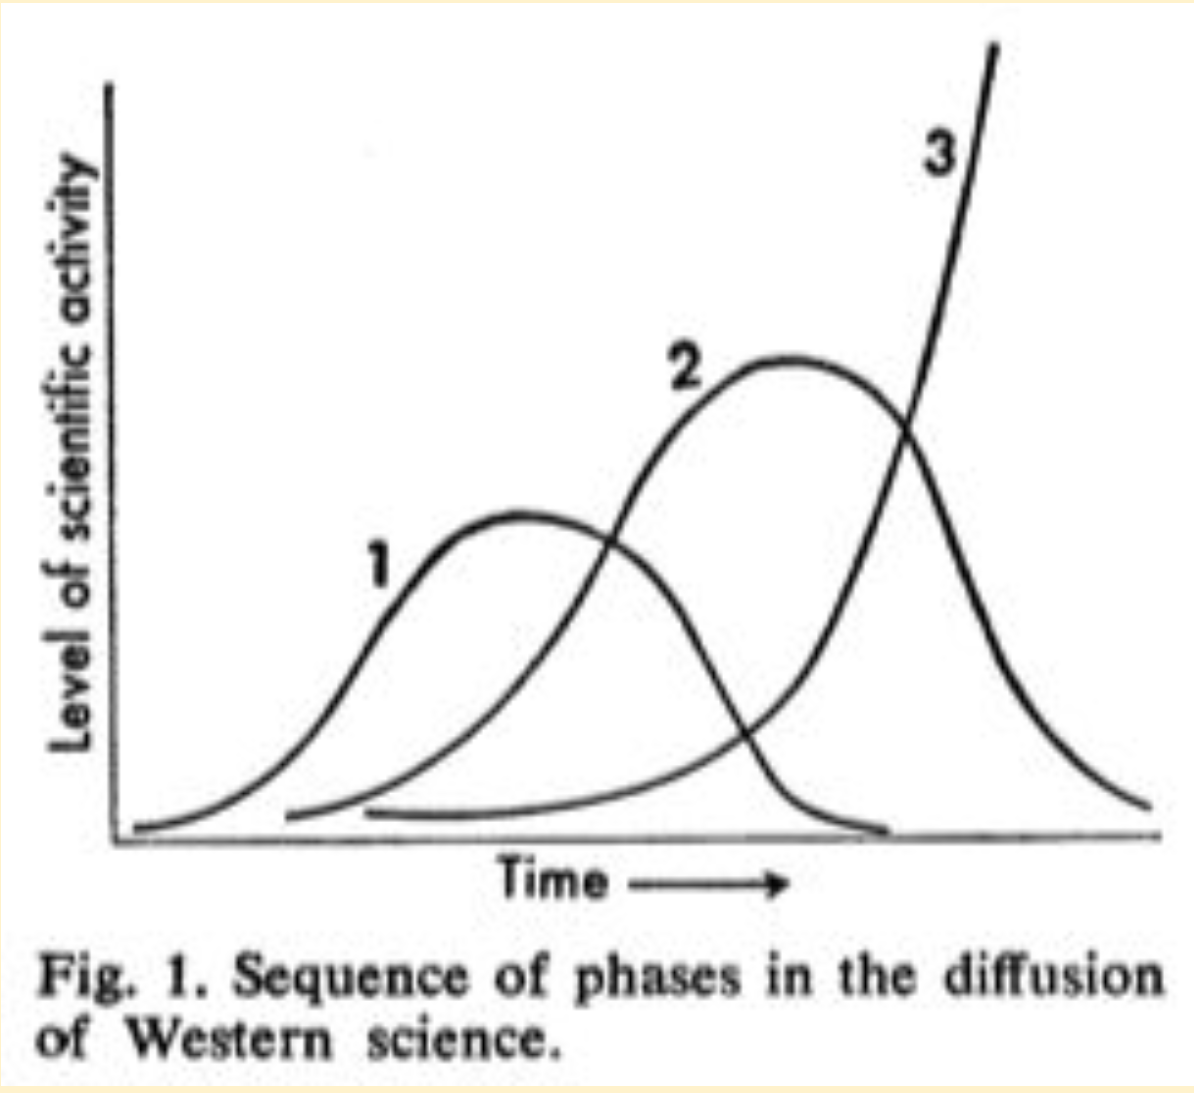
\includegraphics[width=0.5\linewidth]{img/ball's model.PNG}
    \caption[]{Modèle de Basalla \footnote{\cite{ball}} }
    \label{fig:ball_model}
\end{figure}

Nous soutenons l'idée que l'histoire de la science coloniale en Indochine, en général, suit également ce schéma, tout comme le processus de formation et de développement de la Société des Études Indochinoises (S.E.I) et de sa revue.

Si nous appliquons ce modèle au parcours du Bulletin de la Société des Études Indochinoises (B.S.E.I), nous pouvons estimer que la phase 1 correspond aux 18 premières années d'existence de son prédécesseur, le Bulletin du Comité Agricole et Industriel. La deuxième phase s'étend sur une période de 50 ans, de 1883 à 1933, tandis que la troisième phase commence à émerger de manière plus distincte à la fin des années 1960 et se prolonge jusqu'à la fin de la vie de la revue.

Notre étude se concentre sur une analyse temporelle des contenus de ce journal, dans le but d'identifier les principaux sujets scientifiques et de comprendre comment ils ont été présentés et développés au fil du temps. Cette analyse couvre la période allant de 1883 à 1975, année marquant la fin officielle de la publication du journal.

Pour mener à bien cette exploration, nous avons adopté une approche méthodologique basée sur les humanités numériques. Cette méthodologie implique l'utilisation d'outils et de techniques informatiques pour analyser et cartographier la distribution des contenus au sein du corpus, nous permettant ainsi de dégager des tendances et des évolutions dans les sujets scientifiques abordés.

En résumé, notre question de recherche se penche sur l'histoire du journal sur une période considérable, et nous abordons cette exploration avec une approche méthodologique moderne en nous appuyant sur les humanités numériques pour analyser et interpréter les données.

Premièrement, il convient de noter que grâce au développement de la technologie et à la prise de conscience de l'importance de préserver les sources documentaires anciennes, plusieurs projets ont récemment vu le jour pour numériser les sources de données indochinoises, notamment à ma connaissance, le projet \textbf{Vietnamica}\footnote{\cite{bibli}} et le projet \textbf{Patrimoines parrtagés}\footnote{\cite{partage}} entre Bibliothèque nationale de France et Bibliothèque nationale du Vietnam. Toutefois, ces sources restent largement sous-exploitées, notamment en ce qui concerne les recherches à grande échelle utilisant les humanités numériques. Lors de nos recherches de sources de référence pour cette étude, nous n'avons identifié qu'une étude récente menée par Emmanuelle Affidi sur le \textbf{Dong Duong Tap chi} (1913-1919)\footnote{\cite{duong}}, qui représente une tentative de diffusion du discours et de la science occidentale au Tonkin. Cette étude met en lumière les enjeux de l'interculturalité dans le contexte colonial entre savoir et pouvoir (1906-1936).

Cependant, il est important de souligner que ce nombre limité d'études demeure insuffisant pour exploiter pleinement le trésor de données disponible sur l'Indochine, qui comprend plus de 10.000 documents à la Bibliothèque nationale de France (BnF) et 540.000 pages de documents dans le cadre du projet Vietnamica.

Face à cette situation, et forts des compétences acquises au cours de notre spécialisation en humanités numériques, nous sommes convaincus que la recherche sur le Bulletin de la Société des Études Indochinoises (B.S.E.I) constitue le sujet le plus pertinent et approprié que nous puissions entreprendre. Ces recherches, en plus de la création d'un modèle d'alphabétisation multilingue, marquent les premières étapes d'une enquête plus approfondie sur l'histoire coloniale de l'Indochine et les relations entre le Vietnam et la France sur près d'un siècle d'exposition.

Un exemple qui nous a inspirés à entreprendre cette recherche est le projet de numérisation et de publication de l'ensemble des revues de  	
The Polynesian Society  \footnote{\cite{contribu}}, une société savante établie à l'Université d'Auckland, en Nouvelle-Zélande. Fondée en 1892, sa mission initiale était de promouvoir l'étude académique des cultures et des peuples autochtones de Nouvelle-Zélande, en particulier les Māoris, ainsi que d'autres peuples et cultures des îles du Pacifique, à la fois dans le passé et le présent. Pour atteindre cet objectif, la société a principalement utilisé le Journal de la Société Polynésienne, une publication trimestrielle disponible dans plusieurs langues locales et en anglais. Cette revue a été créé dès les premiers jours de la Société et continue d'être publié jusqu'à aujourd'hui.

Les recherches préliminaires sur B.S.E.I visent également à faire connaître cette revue à un vaste public de chercheurs travaillant sur l'Indochine, en mettant en évidence les trésors scientifiques méconnus de l'époque coloniale.

\section{Plan technique}
La figure \ref{fig:diagram} illustre notre schéma de travail pour explorer le corpus et extraire les sujets latents en utilisant une méthode de regroupement de documents. Tout d'abord, les bulletins sous forme d'images sont convertis en format texte à l'aide de Kraken, puis soumis à des techniques de prétraitement du texte, telles que le nettoyage du texte et la tokenisation. L'exploration du corpus implique différentes analyses et statistiques, qu'elles soient de nature temporelle ou spatiale, afin de mieux comprendre le contenu du corpus. La majeure partie de notre travail consiste à identifier les thèmes présents dans les textes. En utilisant des techniques de modélisation thématique telles que Top2Vec, nous parviendrons à identifier les thèmes dominants dans le corpus.

\begin{figure}[H]
    \centering
    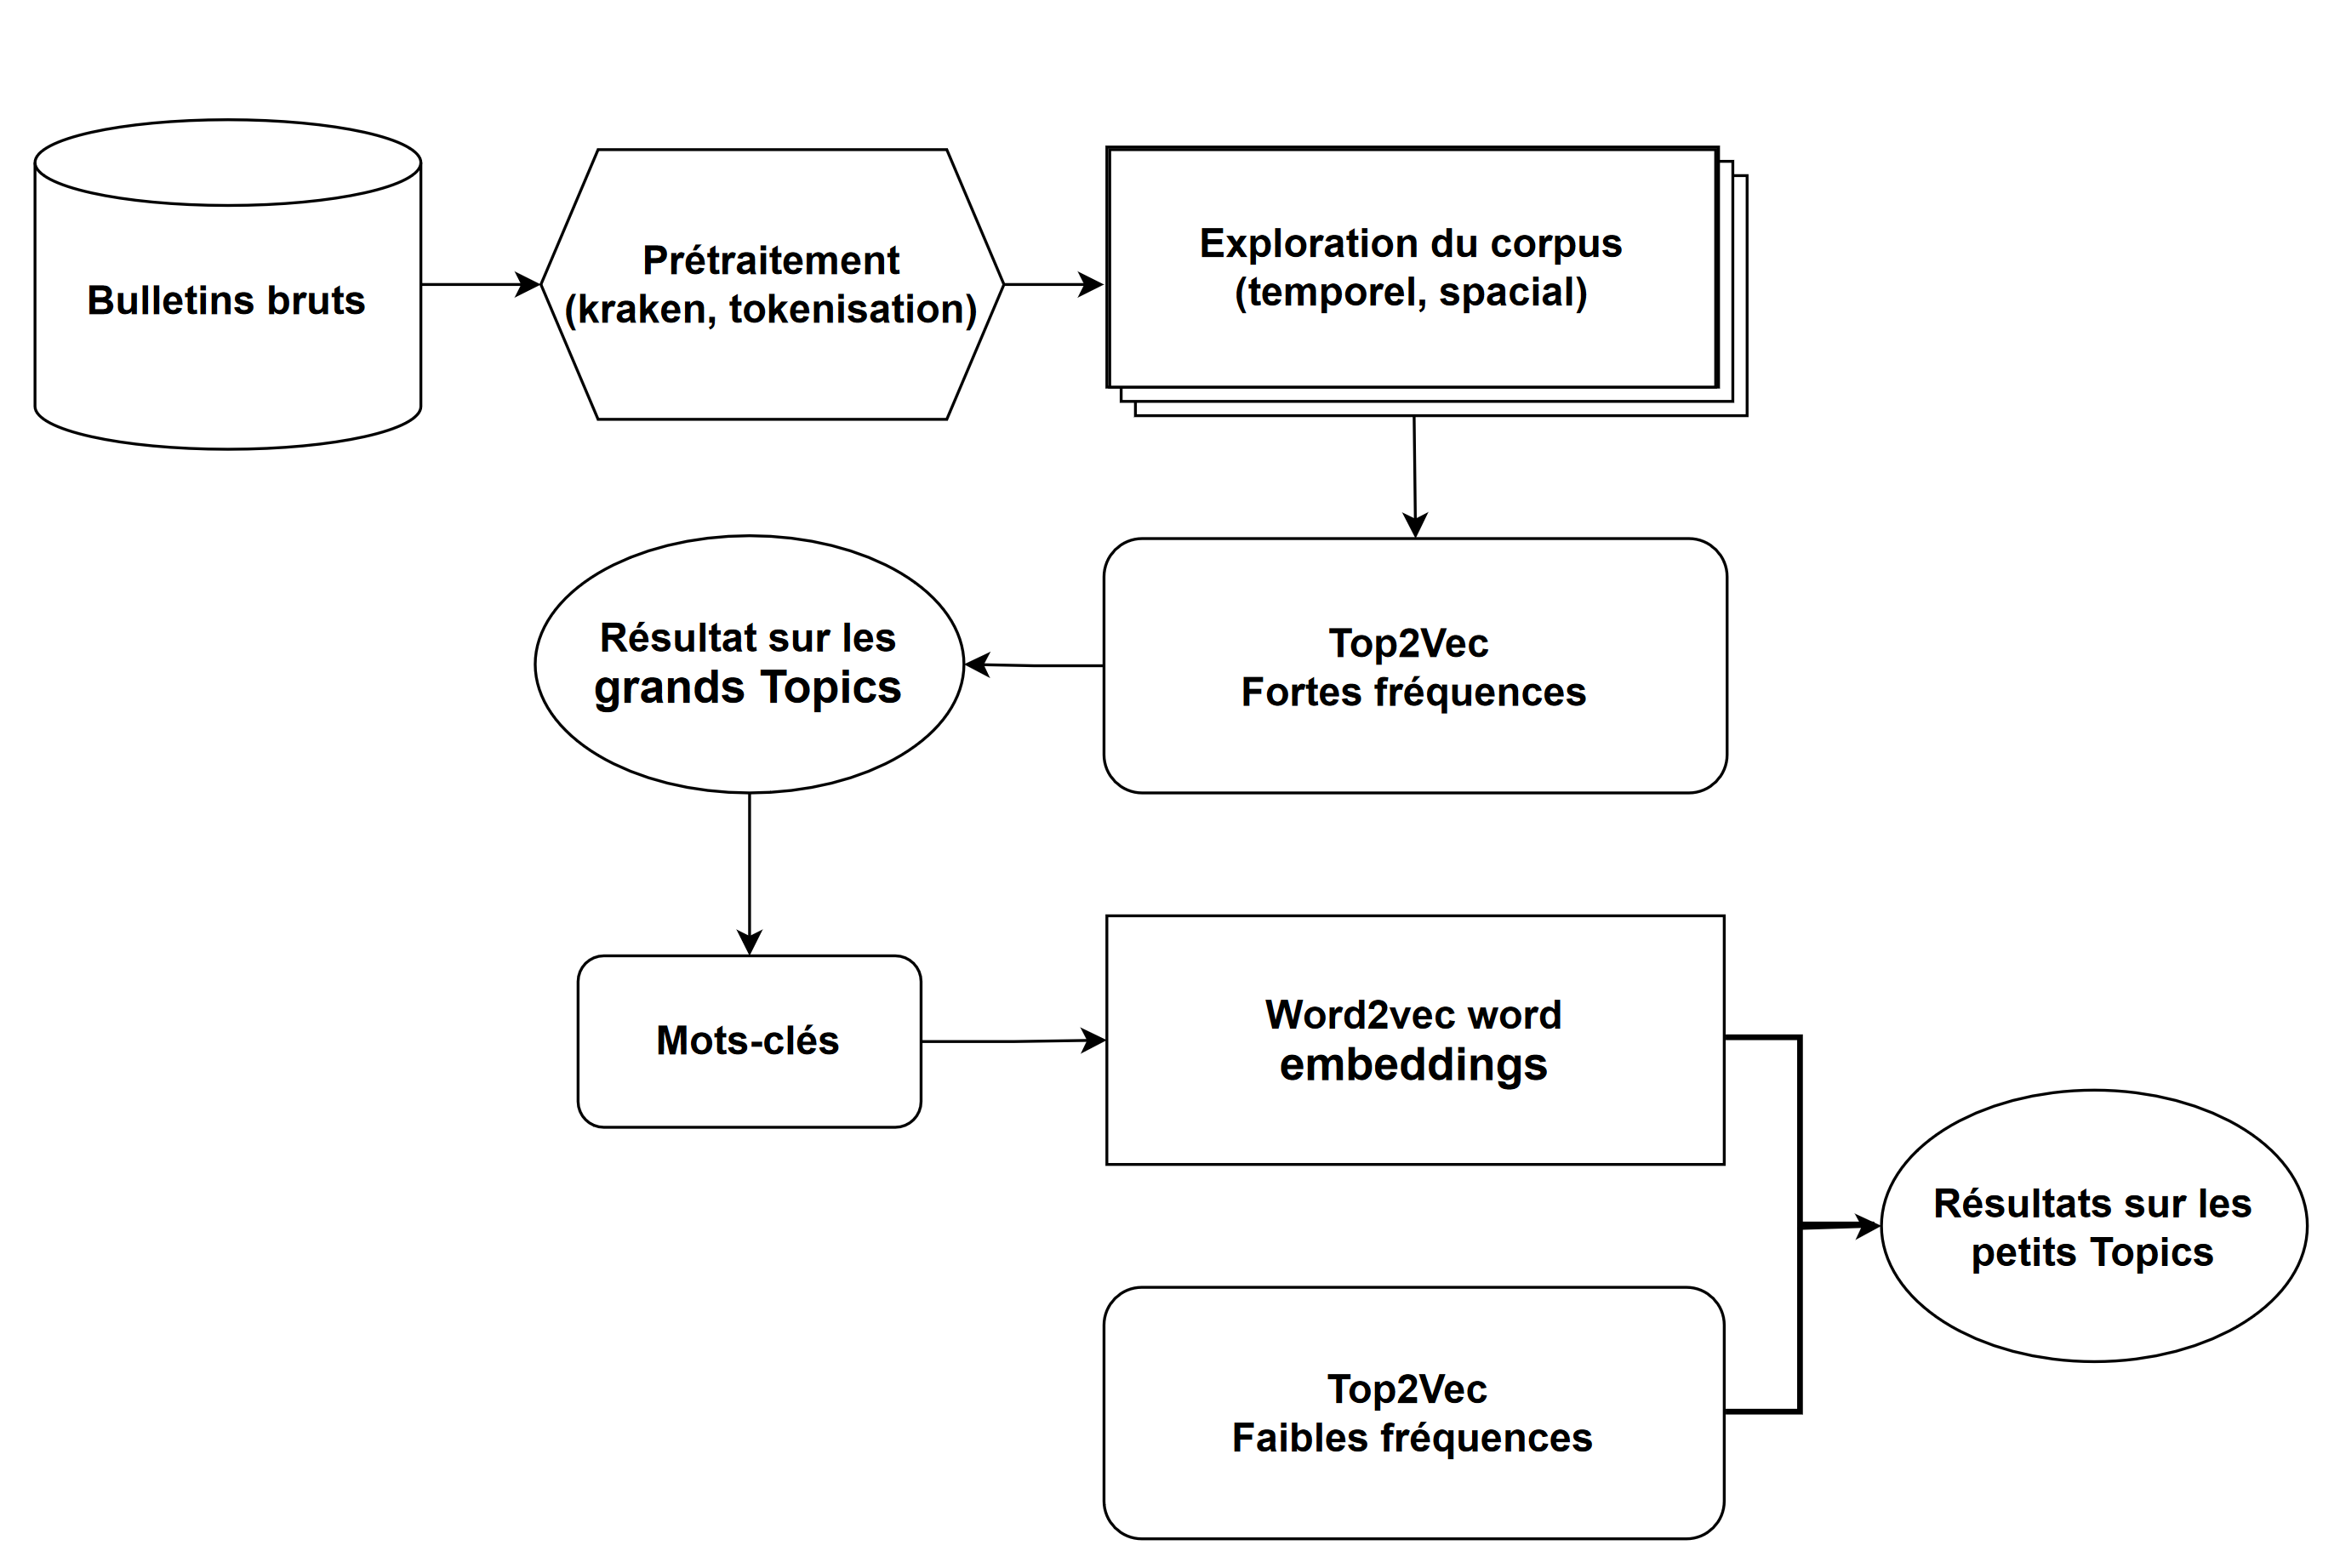
\includegraphics[width=1\linewidth]{img/1.2.diagram.PNG}
    \caption{Diagramme des étapes de travail}
    \label{fig:diagram}
\end{figure}


En premier lieu, le modèle Top2Vec est appliqué aux mots qui apparaissent fréquemment dans le texte, ce qui nous aide à identifier les sujets les plus importants du corpus. Ces sujets sont résumés à l'aide de mots-clés, qui seront ensuite utilisés dans un modèle d'intégration de mots appelé Word2Vec pour créer des ensembles de mots-clés plus détaillés. La combinaison de ces mots-clés avec un modèle Top2Vec entraîné sur des mots à faible fréquence d'occurrence nous permettra d'identifier des groupes de documents contenant des sujets latents à supprimer du corpus.

